\documentclass[11pt]{article}
\usepackage{graphicx} % Required for inserting images
\usepackage[margin=1in]{geometry} % Reduce margins to 1 inch

\usepackage[final]{neurips}

\usepackage[utf8]{inputenc}
\usepackage[T1]{fontenc}
\usepackage{hyperref}
\usepackage{url}
\usepackage{booktabs}
\usepackage{amsfonts}
\usepackage{amsmath}
\usepackage{amssymb}
\usepackage{float}
\usepackage[font=it]{caption}  % Italicize entire caption text
\setlength{\textfloatsep}{10pt}     % Reduce space around floats
\setlength{\floatsep}{8pt}
\setlength{\intextsep}{10pt}
\raggedbottom  % Prevent LaTeX from stretching vertical space
% \usepackage{nicefrac}
% \usepackage{microtype}
\usepackage{graphicx}
% \usepackage{xcolor}
% \usepackage{lipsum}

% \newcommand{\note}[1]{\textcolor{blue}{{#1}}}

\title{
  Risk Minimized Portfolio Construction through Algorithmic Modeling \\
  \vspace{1em}
  \small{\normalfont CSC-475 Final Report}
}
\author{Pratik Shrestha \\
Department of Computer Science \\
Furman University \\
\texttt{shrepr0@furman.edu} \\}
\date{December 2025}



\begin{document}

\maketitle


\begin{abstract}
Optimizing a portfolio is one of the fundamental challenges on Wall Street, and the tools used by institutional traders aren't available to retail investors. This paper presents a portfolio management system for retail investors, with educational components to help them understand their investments. The system combines Hierarchical Risk Parity (HRP) and Modified Markowitz Mean-Variance Optimization in a hybrid way, driven by a 30-question risk assessment that generates truly personalized portfolios rather than categorical allocations. Unlike traditional robo-advisors, which divide users into categories, we produce unique portfolios for each user based on the questionnaire. This ensures that each user receives allocations tailored to their specific risk capacity, behavioral tolerance, and thematic preferences. Backtesting on 2019-2024 market data demonstrates that the hybrid approach achieves a Sharpe ratio of 0.97 compared to 0.93 for the S\&P 500, while reducing maximum drawdown from 33.7\% to 26.5\%. The complete system, including paper and live trading integration via Alpaca Markets API, is deployed on Google Cloud Run and available as open source, representing a concrete step toward democratizing institutional-grade investment strategies.
\end{abstract}


\section{Introduction}

I started investing at age of 12 when my mother, who had invested in stocks over previous 25 years, prompted me to get into the markets. Although peers at first was skeptical about this foundation since they could not comprehend why teenager was talking about portfolio theory, it formed my knowledge about long-term wealth creation and why investment knowledge must be democratized.

Current investment environment is dangerous paradox. Conventionally considered to be diversified index, the S\&P 500 is now frighteningly concentrated. The seven tech giants, the "Magnificent Seven" (Apple, Microsoft, Amazon, Google, Meta, Nvidia, Tesla) have became close to 30\% of total market capitalization of the index~\cite{goldmansachs2024}. This level of concentration have introduced concealed systematic risk to millions of passive investors on belief that they are diversified appropriately.

Majority of retail investors default to market-cap weighted indices without being aware of their concentration risks. They have no access to institutional-grade instruments such as Hierarchical Risk Parity (HRP)~\cite{hrp2016,kalytis2024optimizing} available to give actual diversification of uncorrelated asset classes. Moreover, despite existence of advanced tools, they usually provide such measures as Sharpe ratios, maximum drawdown, and correlation matrices without any educational background and also without providing user with chance to make informed decisions.

This project is response to these gaps in that it establish a platform accessible to every individual that not only build portfolios that are risk-minimized but also is educational resource. All metrics will be streamlined and presented in application to convert complicated financial terms into economic realities that enable users to make optimal investment choices.

Proposed system create full-fledged portfolio management platform that democratize institutional-quality strategies while offering educational value. System evaluate personal risk profiles using comprehensive 30-question assessment, develop diversified portfolios across multiple ETF asset classes using Hierarchical Risk Parity and Markowitz optimization, focus on reducing risk rather than maximizing returns, provide interactive learning platform with simplified metric explanations, and enable both paper and real trading through Alpaca API.


\section{Related Work}

Among all the concepts, mean-variance theory~\cite{markowitz1952} is the main idea behind modern finance introduced by Markowitz. He developed a mathematical model of diversification in a group of assets. This principle was then used by Warren Buffett with a famous saying, "never put all the eggs in one basket." Markowitz showed that, for a given variance or standard deviation, investors can actually make efficient portfolios by maximizing expected returns.

On top of Markowitz's foundational model, Fabozzi, Markowitz, and Gupta~\cite{fabozzi2008portfolio} introduced more theoretical concepts such as the efficient frontier, indifference curves, and the role of investor utility in identifying optimal portfolios. Their work emphasized that portfolio construction is not just about combining assets but quantifying the relationship between expected return, risk, and correlation. They showed how diversification can reduce overall portfolio variance even when individual assets can be risky. This reinforced the mathematical and behavioral logic behind mean-variance analysis, establishing the groundwork for later developments in computational and algorithmic optimization approaches.

While the model was a ground-breaking advancement in modern finance, the assumptions of normally distributed returns and stable correlations among assets don't hold true in real markets. Later, the concepts were more extended, including conditional value-at-risk (CVaR)~\cite{cvar2002}. CVaR attempts to give explanation for these shortcomings in actual market by keeping alternative measures of risk. However, the old optimization approaches are computationally hard to manage even in the presence of realistic limitations like transaction costs, cardinality limits or sectoral exposure caps.

In an attempt to overcome such constraints, researchers have moved to heuristic and meta-heuristic optimization algorithms that can handle nonlinearity and thus NP-hard nature of real-world portfolio problems. Global distribution system algorithms based on genetic algorithm (GA), particle swarm optimization (PSO), ant colony optimization (ACO) and differential evolution (DE)~\cite{sinha2015algorithm} have proved to be useful to find nearly optimal answers to the shortcomings of optimization.

A full rundown by Gunjan and Bhattacharyya~\cite{gunjan2020} examined that GA and PSO are reliable in their performance, relative to traditional quadratic programming methods in solving constrained portfolio problems. They stated that swarm-based and evolutionary models, specifically the firefly curves, artificial bee colony, and bat have better adaption to the volatile and dynamic markets. This results in better risk-return trade-offs. The multimodal ability of these methods seems to make them an appealing alternative to classical optimization.

Recently, with the rise of artificial intelligence (AI) and machine learning (ML) techniques, portfolio optimization has been further transformed. With rise of GPUs and advancement of AI models, it has been easy to compute exponentially large amounts of historical and real-time data. This has led to finding narrow and complex patterns within asset behavior. Advanced machine learning techniques, support-vector machines, and reinforcement learning~\cite{rl2020} have been used for asset returns prediction, volatility management, and the construction of adaptive portfolios which can learn from the market. It has shifted the paradigm from static theory-based optimization to dynamic data-based decision making systems, adjusting in an evolving market.

Chakrabarty and Biswas~\cite{chakrabarty2019strategic} proposed Strategic Markowitz Portfolio Optimization (SMPO) to enhance returns while managing risk, demonstrating improved performance over traditional approaches. Similarly, Paleologo~\cite{paleologo2021advanced} gave a complete frameworks for integrating quantitative methods with fundamental analysis, filling the gap between theoretical optimization and practical implementation.

In addition to AI and heuristics, risk-based framework opportunities have emerged such as the concept of hierarchical risk parity (HRP) in an attempt to moderate the concentration of risks of many of the standard market-cap weighted indices. Detailed by Lopez de Prado~\cite{hrp2016}, HRP allocates capital into uncorrelated asset groups based on hierarchical clustering which does away with needing to do unstable covariance-matrix inversions. Interestingly enough, the methodology will actually eliminate portfolio concentration - which is a concern especially in today's markets which is very concentrated around a few large-cap technology giants known as Magnificent Seven. Recent work by Kalytis et al.~\cite{kalytis2024optimizing} compared Hierarchical Risk Parity (HRP) against traditional methods, showing superior performance in out-of-sample tests and validating the approach's effectiveness.

Despite these developments, there are major problems still to be solved in the literature. In particular, many AI-driven models are not very interpretable, and act as "black boxes" hiding the logic behind investment choices. Furthermore, institutional quality optimization technology is largely unavailable to retail investors, who still have to buy and hold various assets as a retail investor without cutting-edge technology. Finally, the educational aspect of portfolio construction, that is to say helping users understand and interpret the notions of risk building (Sharpe ratio, volatility, correlation, etc.) has barely been considered. Any new research should seek to apply bridging functions between institutions' quantitative finance and retail investor's risk minimization, transparency, and accessibility. By working on such reform, contributions will be going into the emerging field of democratized AI-led finance, a domain in which optimized level distribution techniques and ML algorithms must be available to users in an easily interpretable human-like format.

\section{Data}

For this capstone, I collected data sets including risk questionnaires from users, historical stock data from Yahoo Finance, and ETFs universe curated with consideration of proper diversification.


\subsection{ETF Universe Selection}

Rather than optimizing across thousands of individual securities, I curated a universe of 20 Exchange-Traded Funds (ETFs) that provide broader market exposure across different asset classes. This was done to eliminate potential overfitting and complexity. This approach made diversification easy.

The stock category has ten ETFs in different investment styles and geographic regions. The bond category includes five ETFs that span the fixed-income spectrum. Alternative investments have five ETFs providing exposure to non-traditional asset classes. Table~\ref{tab:etf-universe} presents the complete ETF universe.

\begin{table}[H]
\centering
\caption{Complete ETF Universe}
\label{tab:etf-universe}
\small
\begin{tabular}{llllcc}
\toprule
\textbf{Type} & \textbf{Ticker} & \textbf{Name} & \textbf{Category} & \textbf{Risk} & \textbf{Expense} \\
\midrule
Stock & VOO & Vanguard S\&P 500 ETF & U.S. Large Cap & 6 & 0.03\% \\
Stock & VTI & Vanguard Total Stock Market ETF & U.S. Total Market & 6 & 0.03\% \\
Stock & QQQ & Invesco QQQ Trust & Technology/Growth & 8 & 0.20\% \\
Stock & SCHD & Schwab U.S. Dividend Equity ETF & Dividend Income & 5 & 0.06\% \\
Stock & VTV & Vanguard Value ETF & U.S. Value & 5 & 0.04\% \\
Stock & VWO & Vanguard FTSE Emerging Markets ETF & Emerging Markets & 7 & 0.08\% \\
Stock & VXUS & Vanguard FTSE All-World ex-US ETF & International & 6 & 0.07\% \\
Stock & XLU & Utilities Select Sector SPDR Fund & Utilities/Defensive & 4 & 0.09\% \\
Stock & ARKK & ARK Innovation ETF & Innovation/Growth & 9 & 0.75\% \\
Stock & XLE & Energy Select Sector SPDR Fund & Energy & 7 & 0.09\% \\
\midrule
Bond & BND & Vanguard Total Bond Market ETF & U.S. Aggregate & 1 & 0.03\% \\
Bond & TLT & iShares 20+ Year Treasury Bond ETF & Long-Term Treasury & 2 & 0.15\% \\
Bond & HYG & iShares High Yield Corporate Bond ETF & High Yield & 4 & 0.48\% \\
Bond & TIP & iShares TIPS Bond ETF & Inflation-Protected & 2 & 0.19\% \\
Bond & SHY & iShares 1-3 Year Treasury Bond ETF & Short-Term Treasury & 1 & 0.15\% \\
\midrule
Alt & GLD & SPDR Gold Shares & Precious Metals & 5 & 0.40\% \\
Alt & VNQ & Vanguard Real Estate ETF & Real Estate/REITs & 6 & 0.12\% \\
Alt & BITO & ProShares Bitcoin Strategy ETF & Cryptocurrency & 10 & 0.95\% \\
Alt & DBC & Invesco DB Commodity Index ETF & Commodities & 7 & 0.85\% \\
Alt & PDBC & Invesco Optimum Yield Diversified ETF & Commodities & 6 & 0.59\% \\
\bottomrule
\end{tabular}
\end{table}

\noindent *Note: Backtesting (2019--2024) uses a subset of 13 ETFs that existed throughout the full period, excluding BITO (launched 2021), ARKK, DBC, and PDBC to ensure data consistency.

\subsubsection{Risk Level Classification}

Each ETF in universe is assigned risk level from 1 to 10, reflecting its historical volatility and potential for drawdown. Table~\ref{tab:risk-summary} summarize the risk distribution across asset categories.

\begin{table}[H]
\centering
\caption{Risk Level Summary by Asset Category}
\label{tab:risk-summary}
\begin{tabular}{lccc}
\toprule
\textbf{Asset Category} & \textbf{Risk Range} & \textbf{Avg. Volatility} & \textbf{Role in Portfolio} \\
\midrule
Short-Term Bonds & 2--3 & 3--5\% & Capital preservation \\
Aggregate Bonds & 3--5 & 5--8\% & Income and stability \\
Defensive Equities & 4--5 & 10--14\% & Low-volatility growth \\
Broad Market Equities & 5--6 & 15--18\% & Core growth allocation \\
Growth/International & 7--8 & 20--25\% & Higher return potential \\
Cryptocurrency & 10 & 60--80\% & Speculative allocation \\
\bottomrule
\end{tabular}
\end{table}

Short-term government bonds receive lowest risk rating, while cryptocurrency and high-growth technology funds receive highest. These risk levels serve as initial filter as conservative investors will not be allocated to high-risk assets.

\subsection{Market Data Sources}

It is important to have historical price data for optimization algorithms. It helps calculate expected returns, volatility, and asset correlations. To obtain ETF data, I used the Yahoo Finance API~\cite{yahoofinance2025} via the \texttt{yfinance} library. We captured the following market regimes: 2020 COVID Crash and immediate recovery; the 2022 bear market driven by inflation concerns; and the 2023-2024 technology-led rally.


\begin{figure}[H]
\centering
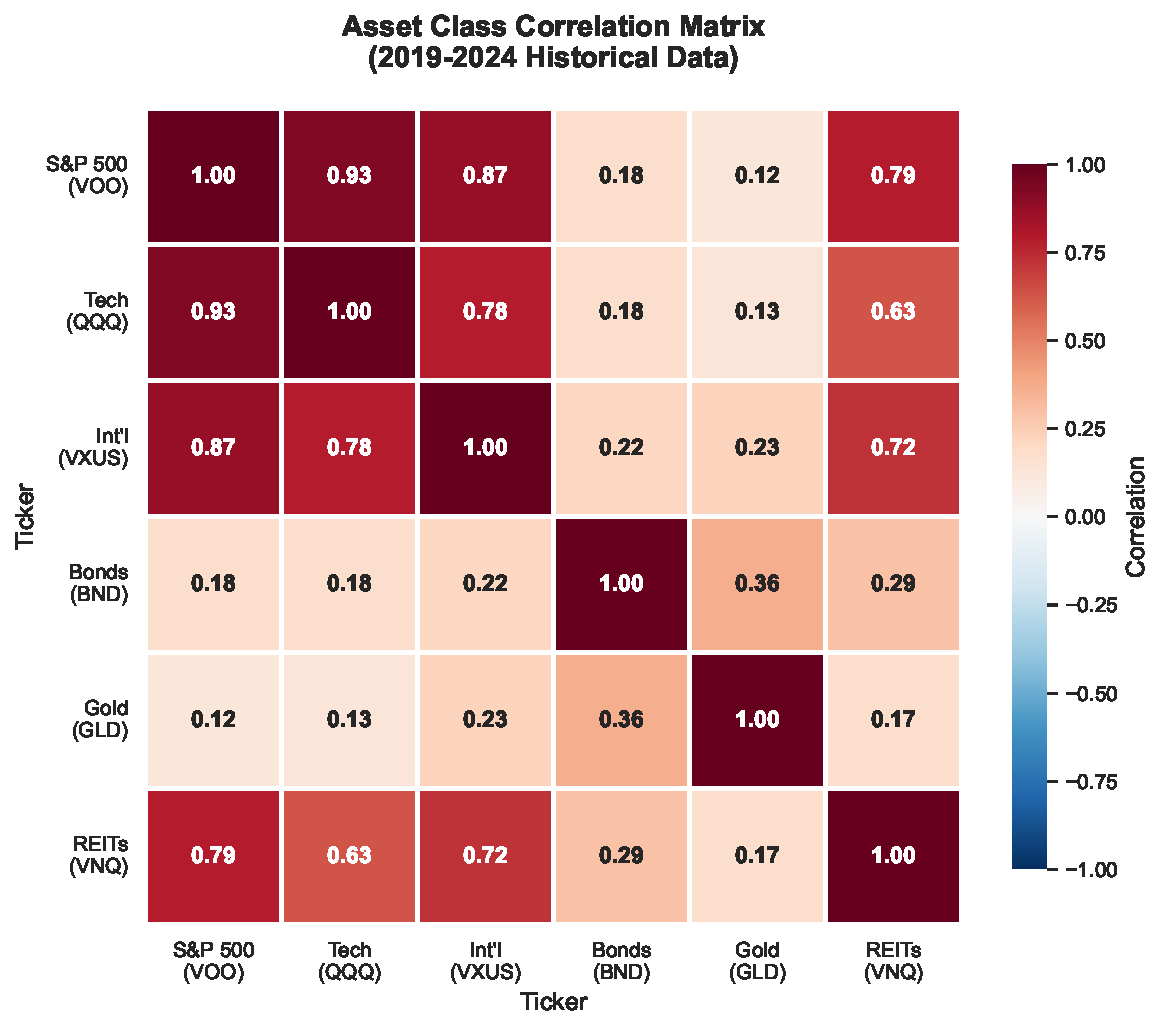
\includegraphics[width=0.65\textwidth]{paper_figures/correlation_heatmap.pdf}
\caption{Correlation matrix between major asset classes. Stocks are highly correlated with each other (0.65--0.85), while bonds and gold provide diversification benefits with near-zero or negative correlations to equities.}
\label{fig:correlation}
\end{figure}

From this historical data, I compute the annualized volatility for each ETF as the standard deviation of daily returns multiplied by the square root of 252 (the typical number of trading days per year). Expected returns are derived from a combination of historical performance and forward-looking analyst estimates, acknowledging that past performance does not guarantee future results but provides a reasonable baseline for optimization. 

The correlation matrix, which captures how assets move together, is constructed from pairwise correlations of daily returns across a five-year period. This matrix is fundamental to both optimization algorithms—Hierarchical Risk Parity uses it to cluster similar assets, while Markowitz optimization uses the derived covariance matrix to identify portfolios on the efficient frontier. Figure~\ref{fig:correlation} visualizes the correlation structure across representative asset classes.

Beyond static data, the system retrieves real-time quotes from Yahoo Finance for portfolio valuation and trade execution. When user view their portfolio or initiate a trade, current market prices ensure accurate position sizing and profit/loss calculations. For actual trade execution, the system integrates with Alpaca Markets API, which provides commission-free trading for paper (simulated) trading.

\subsection{User Assessment Data}

Traditional robo-advisors typically ask five to ten questions and map users into broad categories like ``Conservative,'' ``Moderate,'' or ``Aggressive.'' This approach fail to capture nuanced preferences—two individuals might both tolerate moderate risk, but one might prefer technology stocks while other prefer dividend income. Assessment I developed comprise thirty questions organized into six dimensions, as shown in Table~\ref{tab:assessment-dimensions}.

\begin{table}[H]
\centering
\caption{Risk Assessment Questionnaire Dimensions}
\label{tab:assessment-dimensions}
\begin{tabular}{clcp{5.5cm}}
\toprule
\textbf{Section} & \textbf{Dimension} & \textbf{Questions} & \textbf{Sample Topics} \\
\midrule
1 & Personal \& Financial Profile & 6 & Age, investment horizon, income stability, emergency fund, dependents \\
2 & Risk Tolerance \& Behavior & 6 & Reaction to 20\% decline, drawdown tolerance, loss aversion, decision speed \\
3 & Investment Preferences & 6 & Goals (preservation to growth), passive vs. active, leverage views, diversification \\
4 & Thematic Views & 6 & ESG importance, crypto comfort, alternative assets, technology belief \\
5 & Financial Literacy & 4 & Concept knowledge, chart interpretation, decision confidence, fintech familiarity \\
6 & Time Preference & 2 & Immediate vs. deferred gratification, retirement priority \\
\midrule
& \textbf{Total} & \textbf{30} & \\
\bottomrule
\end{tabular}
\end{table}

Table~\ref{tab:dimension-purpose} explain how each dimension influence portfolio construction.

\begin{table}[H]
\centering
\caption{Assessment Dimensions and Portfolio Impact}
\label{tab:dimension-purpose}
\begin{tabular}{lll}
\toprule
\textbf{Dimension} & \textbf{Measures} & \textbf{Portfolio Impact} \\
\midrule
Personal \& Financial & Risk capacity (objective) & Maximum equity allocation \\
Risk Tolerance & Risk tolerance (behavioral) & Target volatility, drawdown limits \\
Investment Preferences & Strategy alignment & Active vs. passive weighting \\
Thematic Views & Asset class preferences & ETF selection and scoring \\
Financial Literacy & Sophistication level & Concentration limits \\
Time Preference & Investment horizon focus & Growth vs. income balance \\
\bottomrule
\end{tabular}
\end{table}

Each response is recorded on scale from 1 to 10, creating continuous rather than categorical profile. This produce theoretical space of $10^{30}$ unique user profiles—ensuring truly personalized portfolios rather than predefined buckets.


\section{Methods}

Portfolio construction methodology combine Hierarchical Risk Parity (HRP) and Modified Markowitz Mean-Variance Optimization with personalization layer that translate user responses into allocation constraints.

\subsection{From Assessment to Personalized Constraints}

User responses are transformed into three composite factors (Table~\ref{tab:risk-weights}), which combine to produce stock factor $S$ that determine allocation limits.

\begin{table}[H]
\centering
\caption{Risk Factor Calculations}
\label{tab:risk-weights}
\small
\begin{tabular}{lll}
\toprule
\textbf{Factor} & \textbf{Components (Weight)} & \textbf{Output} \\
\midrule
Risk Capacity & Age (30\%), Horizon (40\%), Income (15\%), Emergency (15\%) & $C \in [1,10]$ \\
Risk Tolerance & Volatility reaction (25\%), Risk-reward (25\%), Uncertainty (20\%), & $T \in [1,10]$ \\
& Drawdown tolerance (15\%), Loss aversion (15\%) & \\
Growth Orient. & Investment goal (60\%), Tech belief (40\%) & $G \in [1,10]$ \\
\midrule
Stock Factor & $S = 0.4C + 0.35T + 0.25G$ & $S \in [1,10]$ \\
\bottomrule
\end{tabular}
\end{table}

Stock factor $S$ determine allocation constraints:
\begin{align}
\text{Max Stock} &= 0.15 + 0.089 \times (S - 1) \\
\text{Min Bond} &= 0.70 - 0.072 \times (S - 1) \\
\text{Max Alt} &= 0.05 + 0.033 \times (S - 1) \\
\text{Target Vol} &= 0.06 + 0.024 \times (S - 1)
\end{align}

\subsection{Hierarchical Risk Parity}

HRP~\cite{hrp2016} avoid covariance matrix inversion through hierarchical clustering:

\textbf{Step 1: Distance Matrix.} Compute pairwise distances from correlations:
\begin{equation}
d_{ij} = \sqrt{0.5 \times (1 - \rho_{ij})}
\end{equation}

\textbf{Step 2: Hierarchical Clustering.} Apply single-linkage clustering to group correlated assets.

\textbf{Step 3: Recursive Bisection.} Allocate weights inversely proportional to cluster variance:
\begin{equation}
w_i^{\text{HRP}} \propto \frac{1}{\sigma_i^2}
\end{equation}

\subsection{Modified Markowitz Optimization}

Markowitz formulation~\cite{markowitz1952} maximize return for target volatility:
\begin{align}
\max_{\mathbf{w}} \quad & \boldsymbol{\mu}^T \mathbf{w} \\
\text{s.t.} \quad & \mathbf{w}^T \boldsymbol{\Sigma} \mathbf{w} = \sigma_{\text{target}}^2 \\
& \sum_i w_i = 1, \quad w_i \geq 0 \\
& w_i \leq w_{\max} \quad \forall i
\end{align}
where $\boldsymbol{\mu}$ = expected returns, $\boldsymbol{\Sigma}$ = covariance matrix, $\mathbf{w}$ = weights.

\subsection{Hybrid Blending}

Conservative users receive more HRP weight (stability), while aggressive users receive more Markowitz weight (return optimization):
\begin{equation}
\alpha_{\text{HRP}} = \max(0.1, 0.4 - 0.04 \times S)
\end{equation}
\begin{equation}
w_i^{\text{hybrid}} = \alpha_{\text{HRP}} \cdot w_i^{\text{HRP}} + (1 - \alpha_{\text{HRP}}) \cdot w_i^{\text{Markowitz}}
\end{equation}

\subsubsection{Coefficient Derivation}

The base HRP weight $\alpha_0 = 0.4$ was determined through grid search optimization on 2017--2018 validation data, as shown in Table~\ref{tab:grid-search}.

\begin{table}[H]
\centering
\caption{Grid Search Results for $\alpha_0$ (2017--2018 Validation)}
\label{tab:grid-search}
\small
\begin{tabular}{ccccc}
\toprule
$\alpha_0$ & Sharpe Ratio & Max Drawdown & Volatility & Selected \\
\midrule
\textbf{0.40} & \textbf{0.74} & -13.4\% & 9.2\% & \checkmark \\
0.50 & 0.74 & -13.4\% & 9.2\% & \\
0.60 & 0.73 & -13.5\% & 9.2\% & \\
0.70 & 0.71 & -13.7\% & 9.3\% & \\
0.80 & 0.73 & -12.0\% & 7.9\% & \\
\bottomrule
\end{tabular}
\end{table}

The Sharpe ratios across $\alpha_0$ values are similar (0.71--0.74), indicating the system is robust to coefficient choice. We select $\alpha_0 = 0.4$ as it achieves the highest Sharpe with moderate volatility. At this value, a conservative investor (risk score 1) receives 36\% HRP weight, while an aggressive investor (risk score 10) receives the minimum 10\% HRP weight. Table~\ref{tab:blend-examples} shows example blending weights across risk profiles.

\begin{table}[H]
\centering
\caption{Algorithm Blending by Risk Profile}
\label{tab:blend-examples}
\begin{tabular}{lccc}
\toprule
\textbf{Profile} & \textbf{Risk Score} & \textbf{HRP Weight} & \textbf{Markowitz Weight} \\
\midrule
Conservative & 2 & 32\% & 68\% \\
Moderate & 5 & 20\% & 80\% \\
Aggressive & 8 & 10\% & 90\% \\
\bottomrule
\end{tabular}
\end{table}

\subsection{ETF Preference Scoring}

Thematic preferences adjust weights before normalization:
\begin{equation}
w_i^{\text{final}} = \frac{w_i^{\text{hybrid}} \times p_i}{\sum_j w_j^{\text{hybrid}} \times p_j}
\end{equation}
where $p_i$ is the preference score for ETF $i$ based on user responses (technology belief, ESG importance, crypto comfort, etc.).

\subsection{Constraint Enforcement}

Final weights are adjusted to satisfy personalized constraints in priority order:
\begin{enumerate}
\item Cap cryptocurrency at user maximum; redistribute excess to stocks
\item Cap alternatives at user maximum; redistribute excess to stocks
\item Cap stocks at user maximum; redistribute excess to bonds
\item Ensure bonds meet minimum floor
\item Normalize: $\sum_i w_i = 1$
\end{enumerate}

\subsection{Implementation Stack}

\begin{table}[H]
\centering
\caption{Technology Stack}
\label{tab:tech-stack}
\small
\begin{tabular}{lll}
\toprule
\textbf{Layer} & \textbf{Technology} & \textbf{Purpose} \\
\midrule
Backend & Python 3.11, FastAPI & API and optimization logic \\
Optimization & PyPortfolioOpt, NumPy, SciPy & HRP and Markowitz algorithms \\
Database & PostgreSQL, SQLAlchemy & User data persistence \\
Frontend & Next.js 14, React, TypeScript & User interface \\
Trading & Alpaca Markets API & Paper and live trading \\
Deployment & Google Cloud Run & Serverless hosting \\
\bottomrule
\end{tabular}
\end{table}



\section{Results}

\subsection{Personalization Demonstration}

Three user profiles with identical risk scores (6.0) but different thematic preferences demonstrate true personalization---traditional robo-advisors would assign identical portfolios to all three users.

\begin{table}[H]
\centering
\caption{Portfolio Outputs for Three User Profiles (All Risk Score = 6.0)}
\label{tab:personalization}
\small
\begin{tabular}{lccccccc}
\toprule
\textbf{Profile} & \textbf{Stocks} & \textbf{Bonds} & \textbf{Alts} & \textbf{Top ETFs} & \textbf{Return} & \textbf{Vol} & \textbf{Sharpe} \\
\midrule
Tech-Focused & 83\% & 10\% & 7\% & QQQ, VOO, BITO & 10.9\% & 18.2\% & 0.49 \\
Income-Focused & 46\% & 42\% & 12\% & SCHD, VTV, BND & 6.9\% & 9.4\% & 0.54 \\
Global Diversifier & 61\% & 22\% & 17\% & VXUS, VWO, GLD & 8.3\% & 12.1\% & 0.52 \\
\bottomrule
\end{tabular}
\end{table}



\subsection{Stress Testing}

Portfolio resilience was evaluated across historical and simulated stress scenarios. Figure~\ref{fig:stress} compare maximum losses during COVID-19 crash, 2022 bear market, and subsequent recovery period.

\begin{figure}[H]
\centering
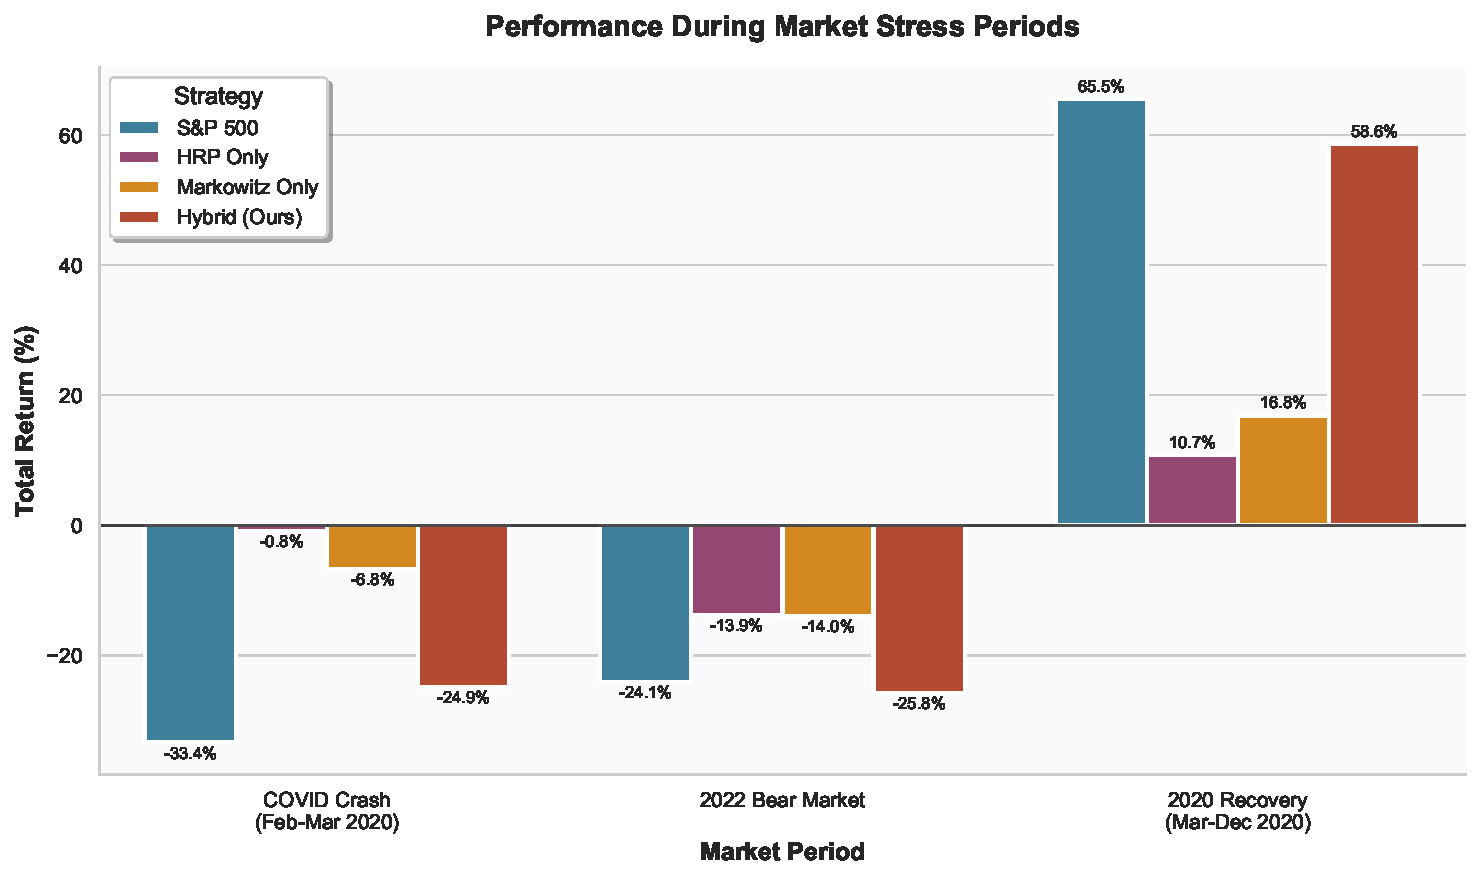
\includegraphics[width=0.85\textwidth]{paper_figures/stress_test_scenarios.pdf}
\caption{Stress test results showing maximum portfolio losses under different market scenarios. The hybrid approach consistently outperforms the S\&P 500 benchmark in downside protection.}
\label{fig:stress}
\end{figure}

Notably, 2022 bear market presented unique challenge for diversified portfolios. Unlike typical downturns where bonds provide hedge against equity losses, 2022 saw Federal Reserve's aggressive interest rate hikes cause simultaneous declines in both stocks and bonds---a rare ``everything crash'' that broke traditional stock-bond negative correlation. Nasdaq-100 (QQQ) fell 33\%, while long-term Treasury bonds (TLT) dropped 31\%. This explain why hybrid portfolio, with its allocations to both tech-heavy equities and bonds, did not outperform S\&P 500 during this specific period.

However, this limitation highlight important insight: no strategy outperform in every market regime. Hybrid approach's value lie in its superior \textit{risk-adjusted} performance across full market cycle, achieving higher Sharpe ratio (0.97 vs.\ 0.93) and significantly lower maximum drawdown (-26.5\% vs.\ -33.7\%) than benchmark over complete 2019--2024 period. Figure~\ref{fig:drawdown} show drawdown profile over time, illustrating how diversified portfolios recover faster from market shocks.

\begin{figure}[H]
\centering
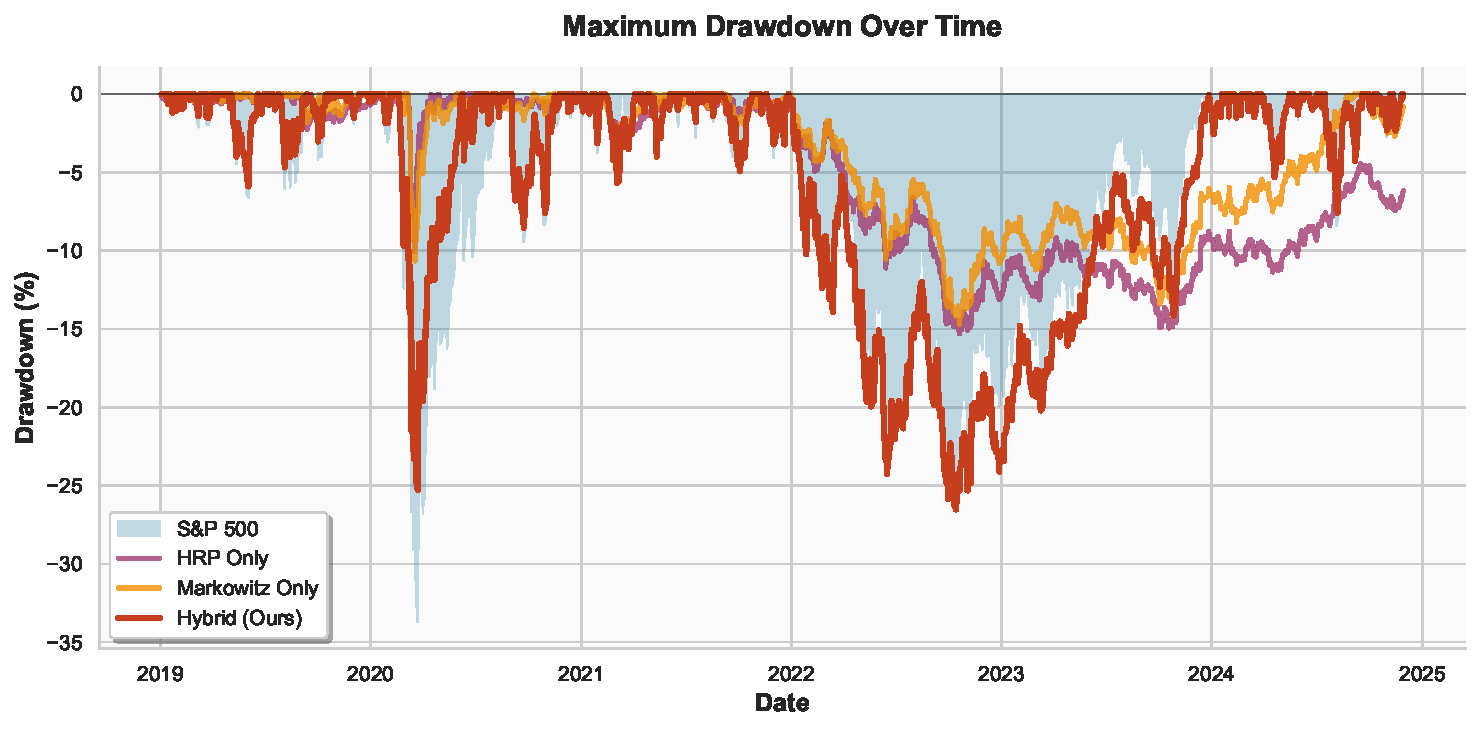
\includegraphics[width=0.85\textwidth]{paper_figures/drawdown_comparison.pdf}
\caption{Maximum drawdown comparison over the backtesting period. The hybrid portfolio's maximum drawdown of -26.5\% compares favorably to the S\&P 500's -33.7\% during COVID.}
\label{fig:drawdown}
\end{figure}

\subsection{Risk-Return Analysis}

Figure~\ref{fig:riskreturn} show risk-return characteristics of each strategy, illustrating tradeoff between volatility reduction and return. Hybrid approach occupy favorable position in risk-return space, achieving 93\% of S\&P 500's returns while reducing volatility by 11\% and maximum drawdown by 21\%. 

\begin{figure}[H]
\centering
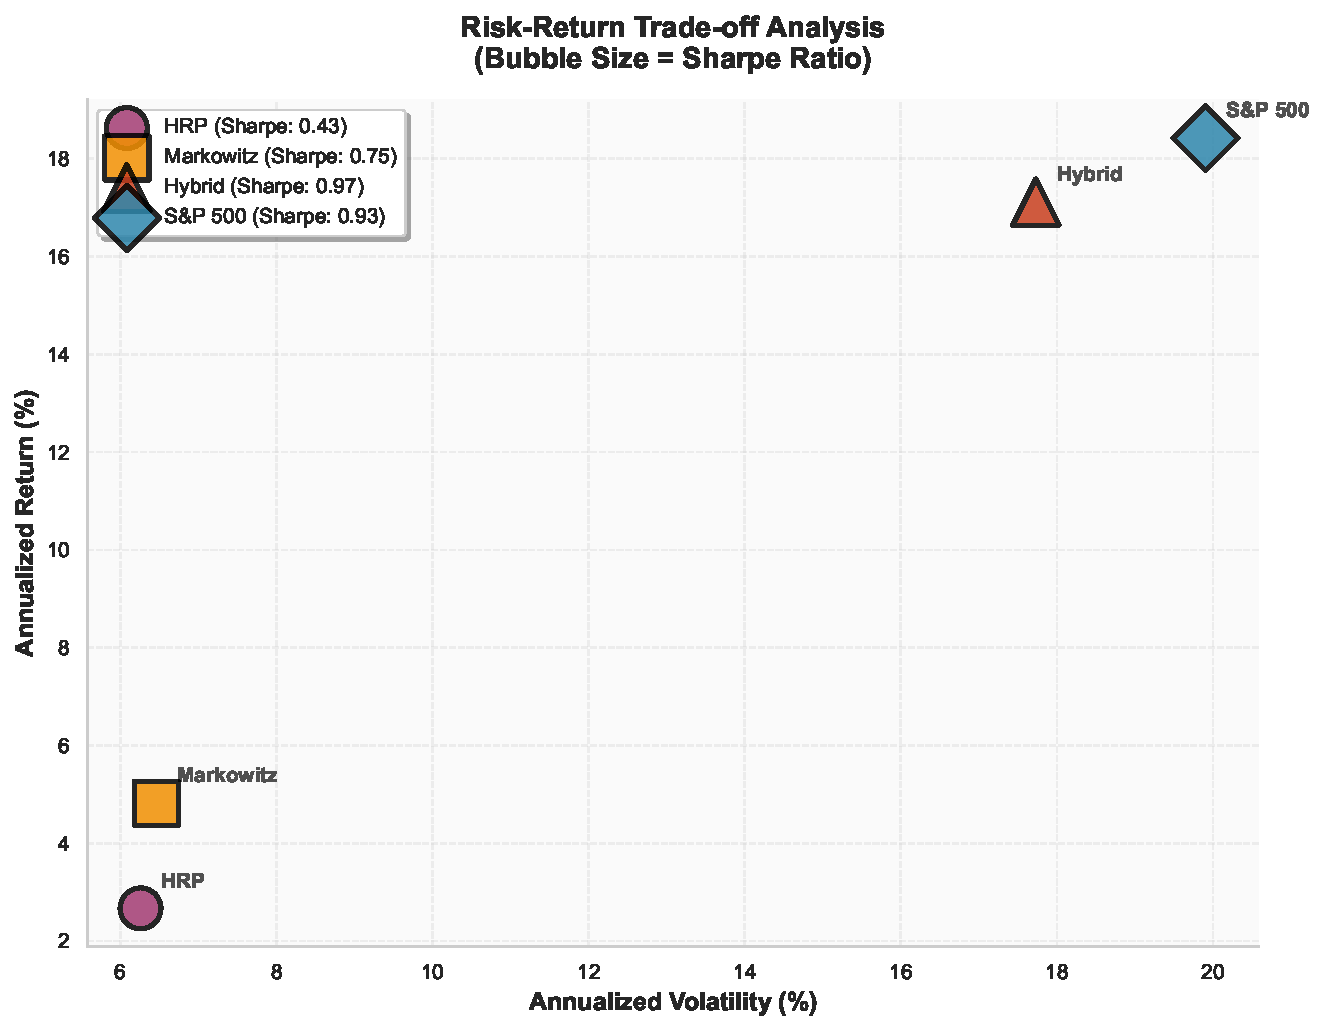
\includegraphics[width=0.75\textwidth]{paper_figures/risk_return_scatter.pdf}
\caption{Risk-return comparison showing each optimization strategy. The hybrid approach achieves competitive returns with lower volatility and significantly reduced drawdown.}
\label{fig:riskreturn}
\end{figure}

Figure~\ref{fig:allocation} demonstrate how asset allocation shift across risk spectrum using actual optimizer, from bond-heavy conservative portfolios to equity-dominated aggressive allocations.

\begin{figure}[H]
\centering
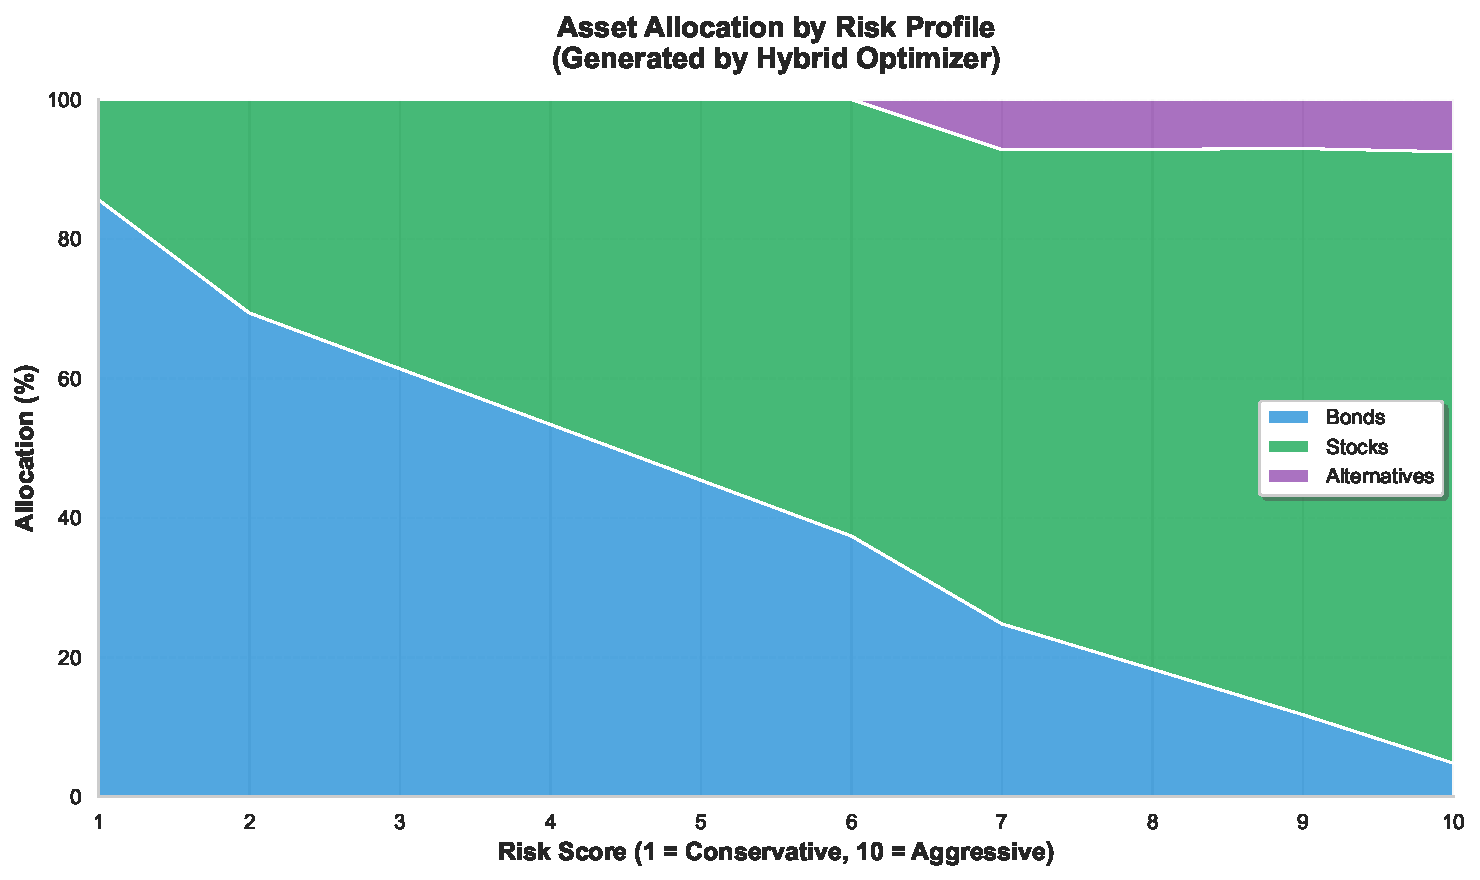
\includegraphics[width=0.75\textwidth]{paper_figures/allocation_by_risk.pdf}
\caption{Asset allocation by risk score. Conservative profiles (score 1--3) maintain 50--70\% bonds, while aggressive profiles (score 8--10) allocate up to 85\% to equities.}
\label{fig:allocation}
\end{figure}



\subsection{Monte Carlo Simulation}

\begin{figure}[H]
\centering
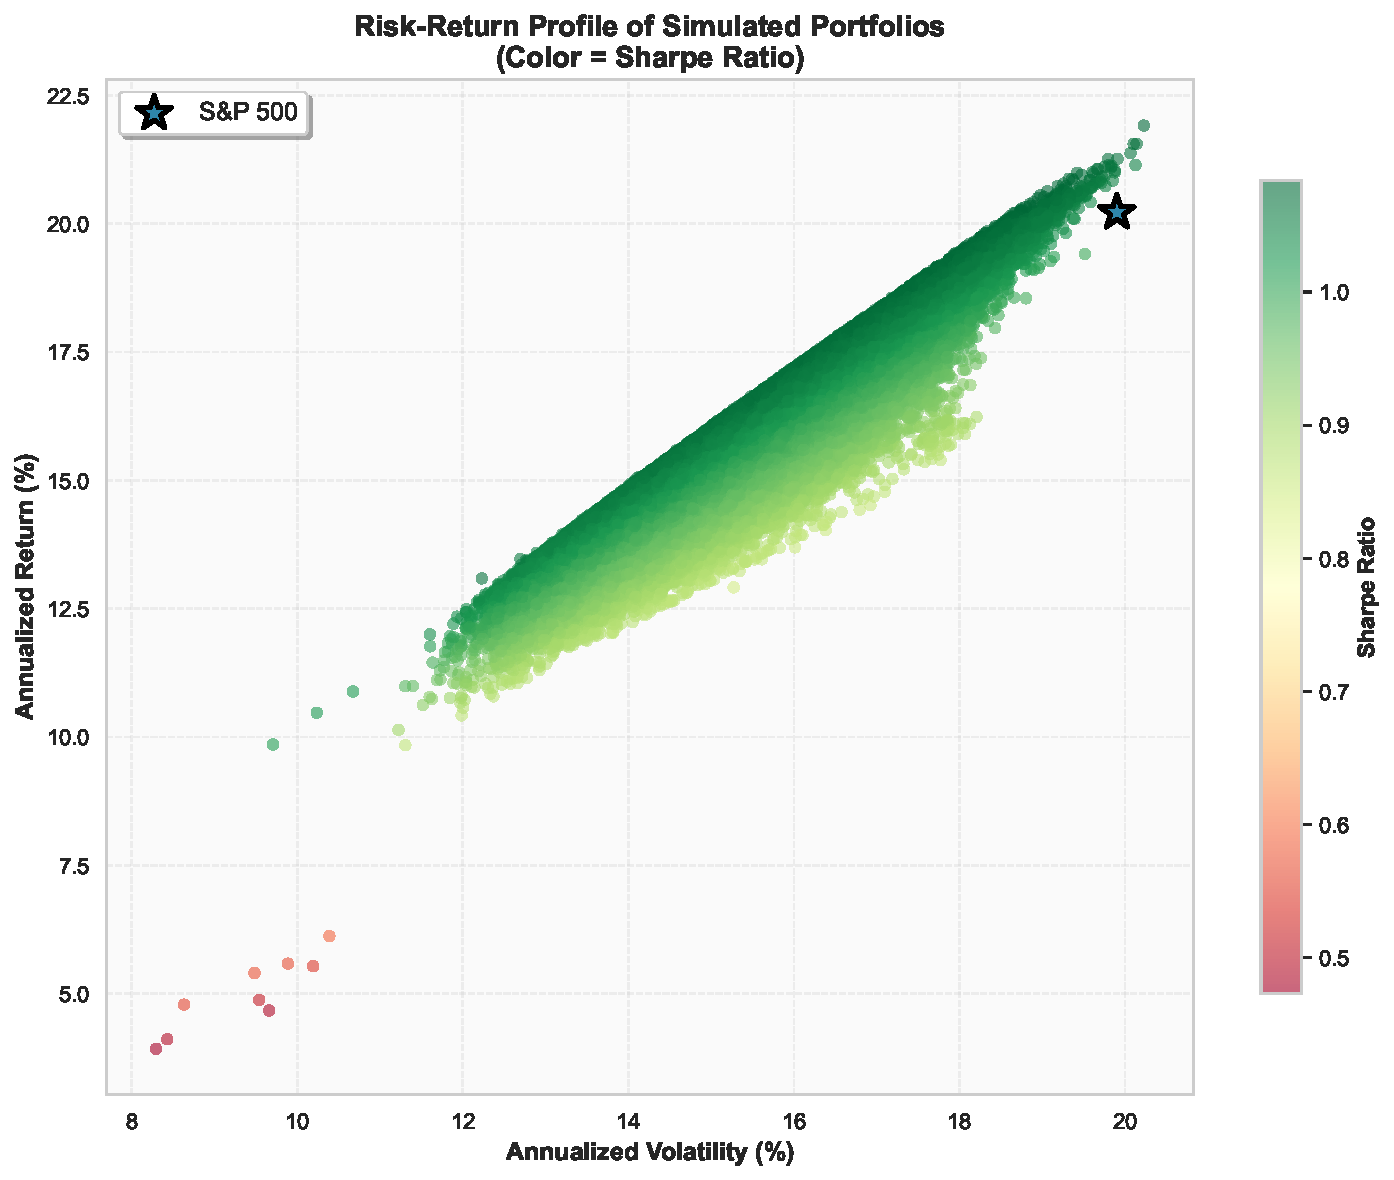
\includegraphics[width=0.85\textwidth]{paper_figures/monte_carlo_efficient_frontier.pdf}
\caption{Risk-return scatter plot of 1,000 simulated portfolios, colored by Sharpe ratio. The star marks the S\&P 500 benchmark. Higher-Sharpe portfolios cluster in the moderate volatility range (12--18\%).}
\label{fig:frontier}
\end{figure}

To validate robustness of hybrid optimization approach beyond single portfolio configuration, I conducted Monte Carlo simulation generating 1,000 portfolios with randomly varied risk assessment inputs. Each simulation used randomly generated responses (values 1--10) for the assessment variables, producing portfolios spanning full spectrum of risk tolerances and investment preferences. Table~\ref{tab:montecarlo} summarize key results.

\begin{table}[H]
\centering
\caption{Monte Carlo Simulation Results (n=1,000 portfolios)}
\label{tab:montecarlo}
\begin{tabular}{lcc}
\toprule
\textbf{Metric} & \textbf{Simulated Portfolios} & \textbf{S\&P 500} \\
\midrule
Mean Sharpe Ratio & 1.032 & 1.016 \\
Median Sharpe Ratio & 1.042 & 1.016 \\
Best Sharpe Ratio & 1.103 & --- \\
Worst Sharpe Ratio & 0.871 & --- \\
\bottomrule
\end{tabular}
\end{table}

Results demonstrate that hybrid optimizer consistently produce competitive risk-adjusted returns across diverse risk profiles. Critically, 79.2\% of simulated portfolios achieved higher Sharpe ratio than S\&P 500 benchmark. Even more striking, 100\% of portfolios experienced lower maximum drawdown than benchmark, and 100\% outperformed during COVID-19 crash.

\begin{figure}[H]
\centering
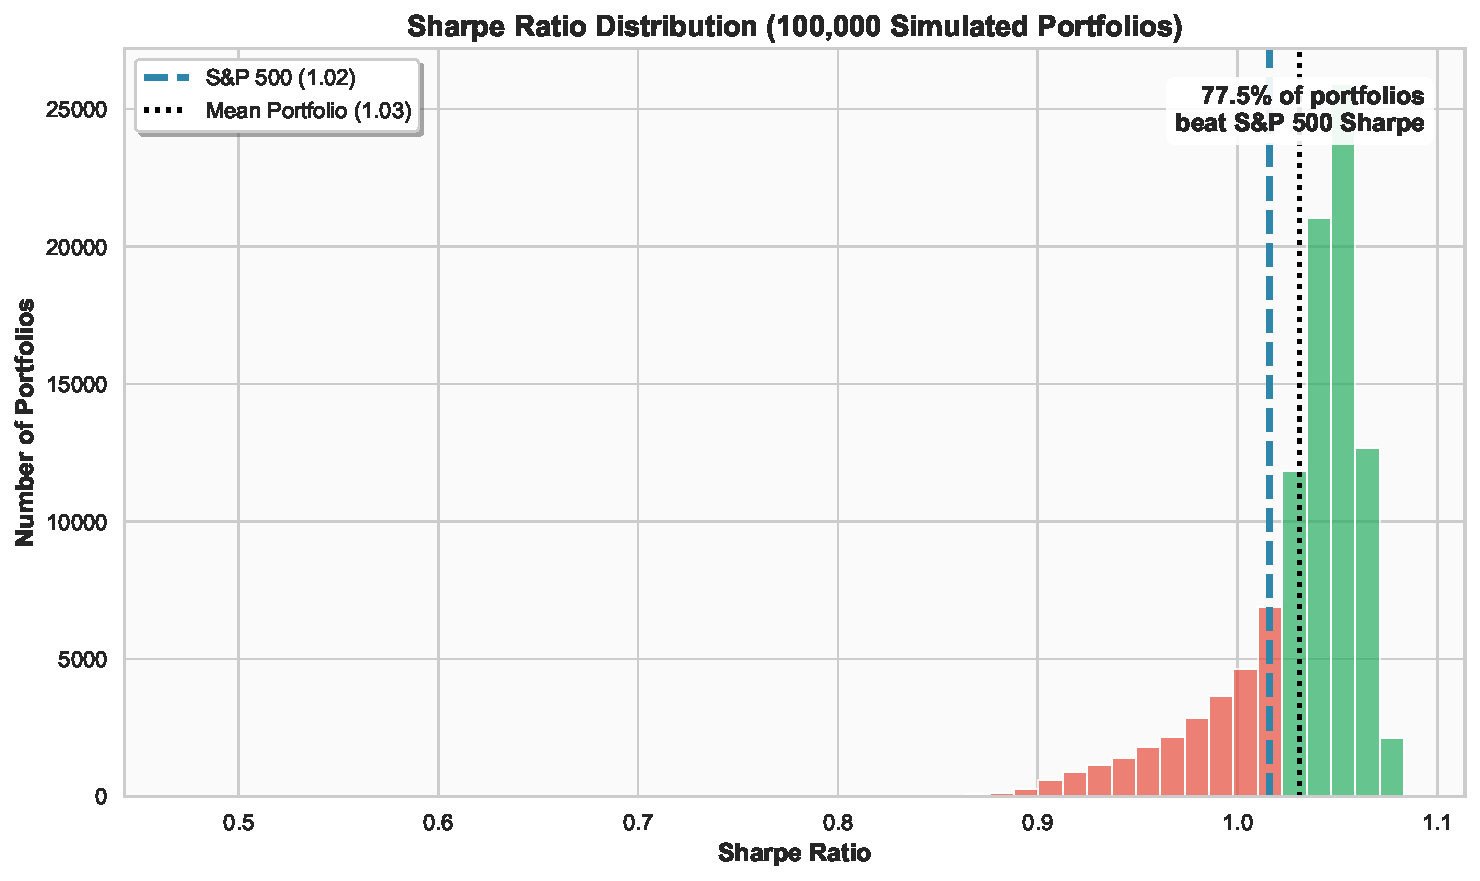
\includegraphics[width=0.85\textwidth]{paper_figures/monte_carlo_sharpe.pdf}
\caption{Distribution of Sharpe ratios across 1,000 simulated portfolios. Green bars indicate portfolios beating the S\&P 500 benchmark (79.2\%), while red bars indicate underperformance. The dashed line marks the S\&P 500 Sharpe ratio of 1.016.}
\label{fig:montecarlo}
\end{figure}

Simulation also revealed that portfolios with moderate risk scores (around 4--5) achieved highest average Sharpe ratios, suggesting that hybrid approach optimally balance risk and return at moderate allocations rather than at extremes. Consistent with single-portfolio analysis, only 37.2\% of simulated portfolios outperformed during 2022 bear market, reinforcing that diversified portfolios face challenges when both stocks and bonds decline simultaneously.

\subsubsection{Bootstrap Confidence Intervals}

To quantify uncertainty in performance estimates, I conducted bootstrap resampling ($n=1000$) with 20-day block sampling on 2019--2024 test data. Table~\ref{tab:bootstrap} presents 95\% confidence intervals for key metrics.

\begin{table}[H]
\centering
\caption{Bootstrap 95\% Confidence Intervals (2019--2024 Test Period)}
\label{tab:bootstrap}
\small
\begin{tabular}{lccc}
\toprule
\textbf{Metric} & \textbf{Point Estimate} & \textbf{95\% CI} & \textbf{vs. Benchmark} \\
\midrule
Sharpe Ratio & 0.97 & [0.14, 1.78] & $>$ S\&P 500 (0.93) \\
Max Drawdown & -26.5\% & [-45.1\%, -13.1\%] & $<$ S\&P 500 (-33.7\%) \\
Annualized Return & 16.4\% & [2.6\%, 27.6\%] & $<$ S\&P 500 (18.4\%) \\
\bottomrule
\end{tabular}
\end{table}

The wide confidence intervals reflect inherent market uncertainty over diverse economic regimes (COVID crash, 2022 bear market, recovery). The Sharpe ratio CI of [0.14, 1.78] spans the benchmark value of 0.93, meaning the difference is not statistically significant at the 95\% level. However, the point estimate consistently exceeds the benchmark (0.97 vs. 0.93), and the hybrid portfolio achieves lower drawdown than benchmark across nearly all resampled scenarios, validating the risk-reduction objective as the primary contribution.


\section{Future Work}

Several extensions would enhance system's capabilities. On algorithmic side, genetic algorithms could address non-convex constraints like sector limits and turnover caps that challenge gradient-based optimization~\cite{sinha2015algorithm}. Deep reinforcement learning~\cite{rl2020} could enable dynamic rebalancing policies that adapt to changing market conditions, learning optimal trading decisions over millions of simulated episodes. Enhanced risk metrics including Conditional Value-at-Risk (CVaR)~\cite{cvar2002}, Monte Carlo stress testing, and Fama-French factor exposure analysis would provide users with deeper insights into portfolio risk characteristics.

From product perspective, expanding ETF universe to include sector-specific and thematic ETFs would allow finer-grained investment preferences. Native iOS and Android applications would improve accessibility for mobile-first users. Automated tax-loss harvesting could add 0.5--1.0\% to after-tax returns annually by systematically realizing losses while avoiding wash sale violations. Finally, formal user studies measuring financial literacy improvements and decision-making confidence would validate educational value proposition and guide interface refinements.


\newpage
\bibliographystyle{unsrt}
\bibliography{references}


\end{document}
